\documentclass{standalone}
\usepackage{tikz}
\usepackage{graphicx}
\usepackage{xcolor}
\usepackage{anyfontsize}

\definecolor{yell}{HTML}{ffde59}
\definecolor{oran}{HTML}{fb7e00}

\begin{document}
\begin{tikzpicture}[scale=1, transform shape]
	\node [anchor=south west] at (0, 0) {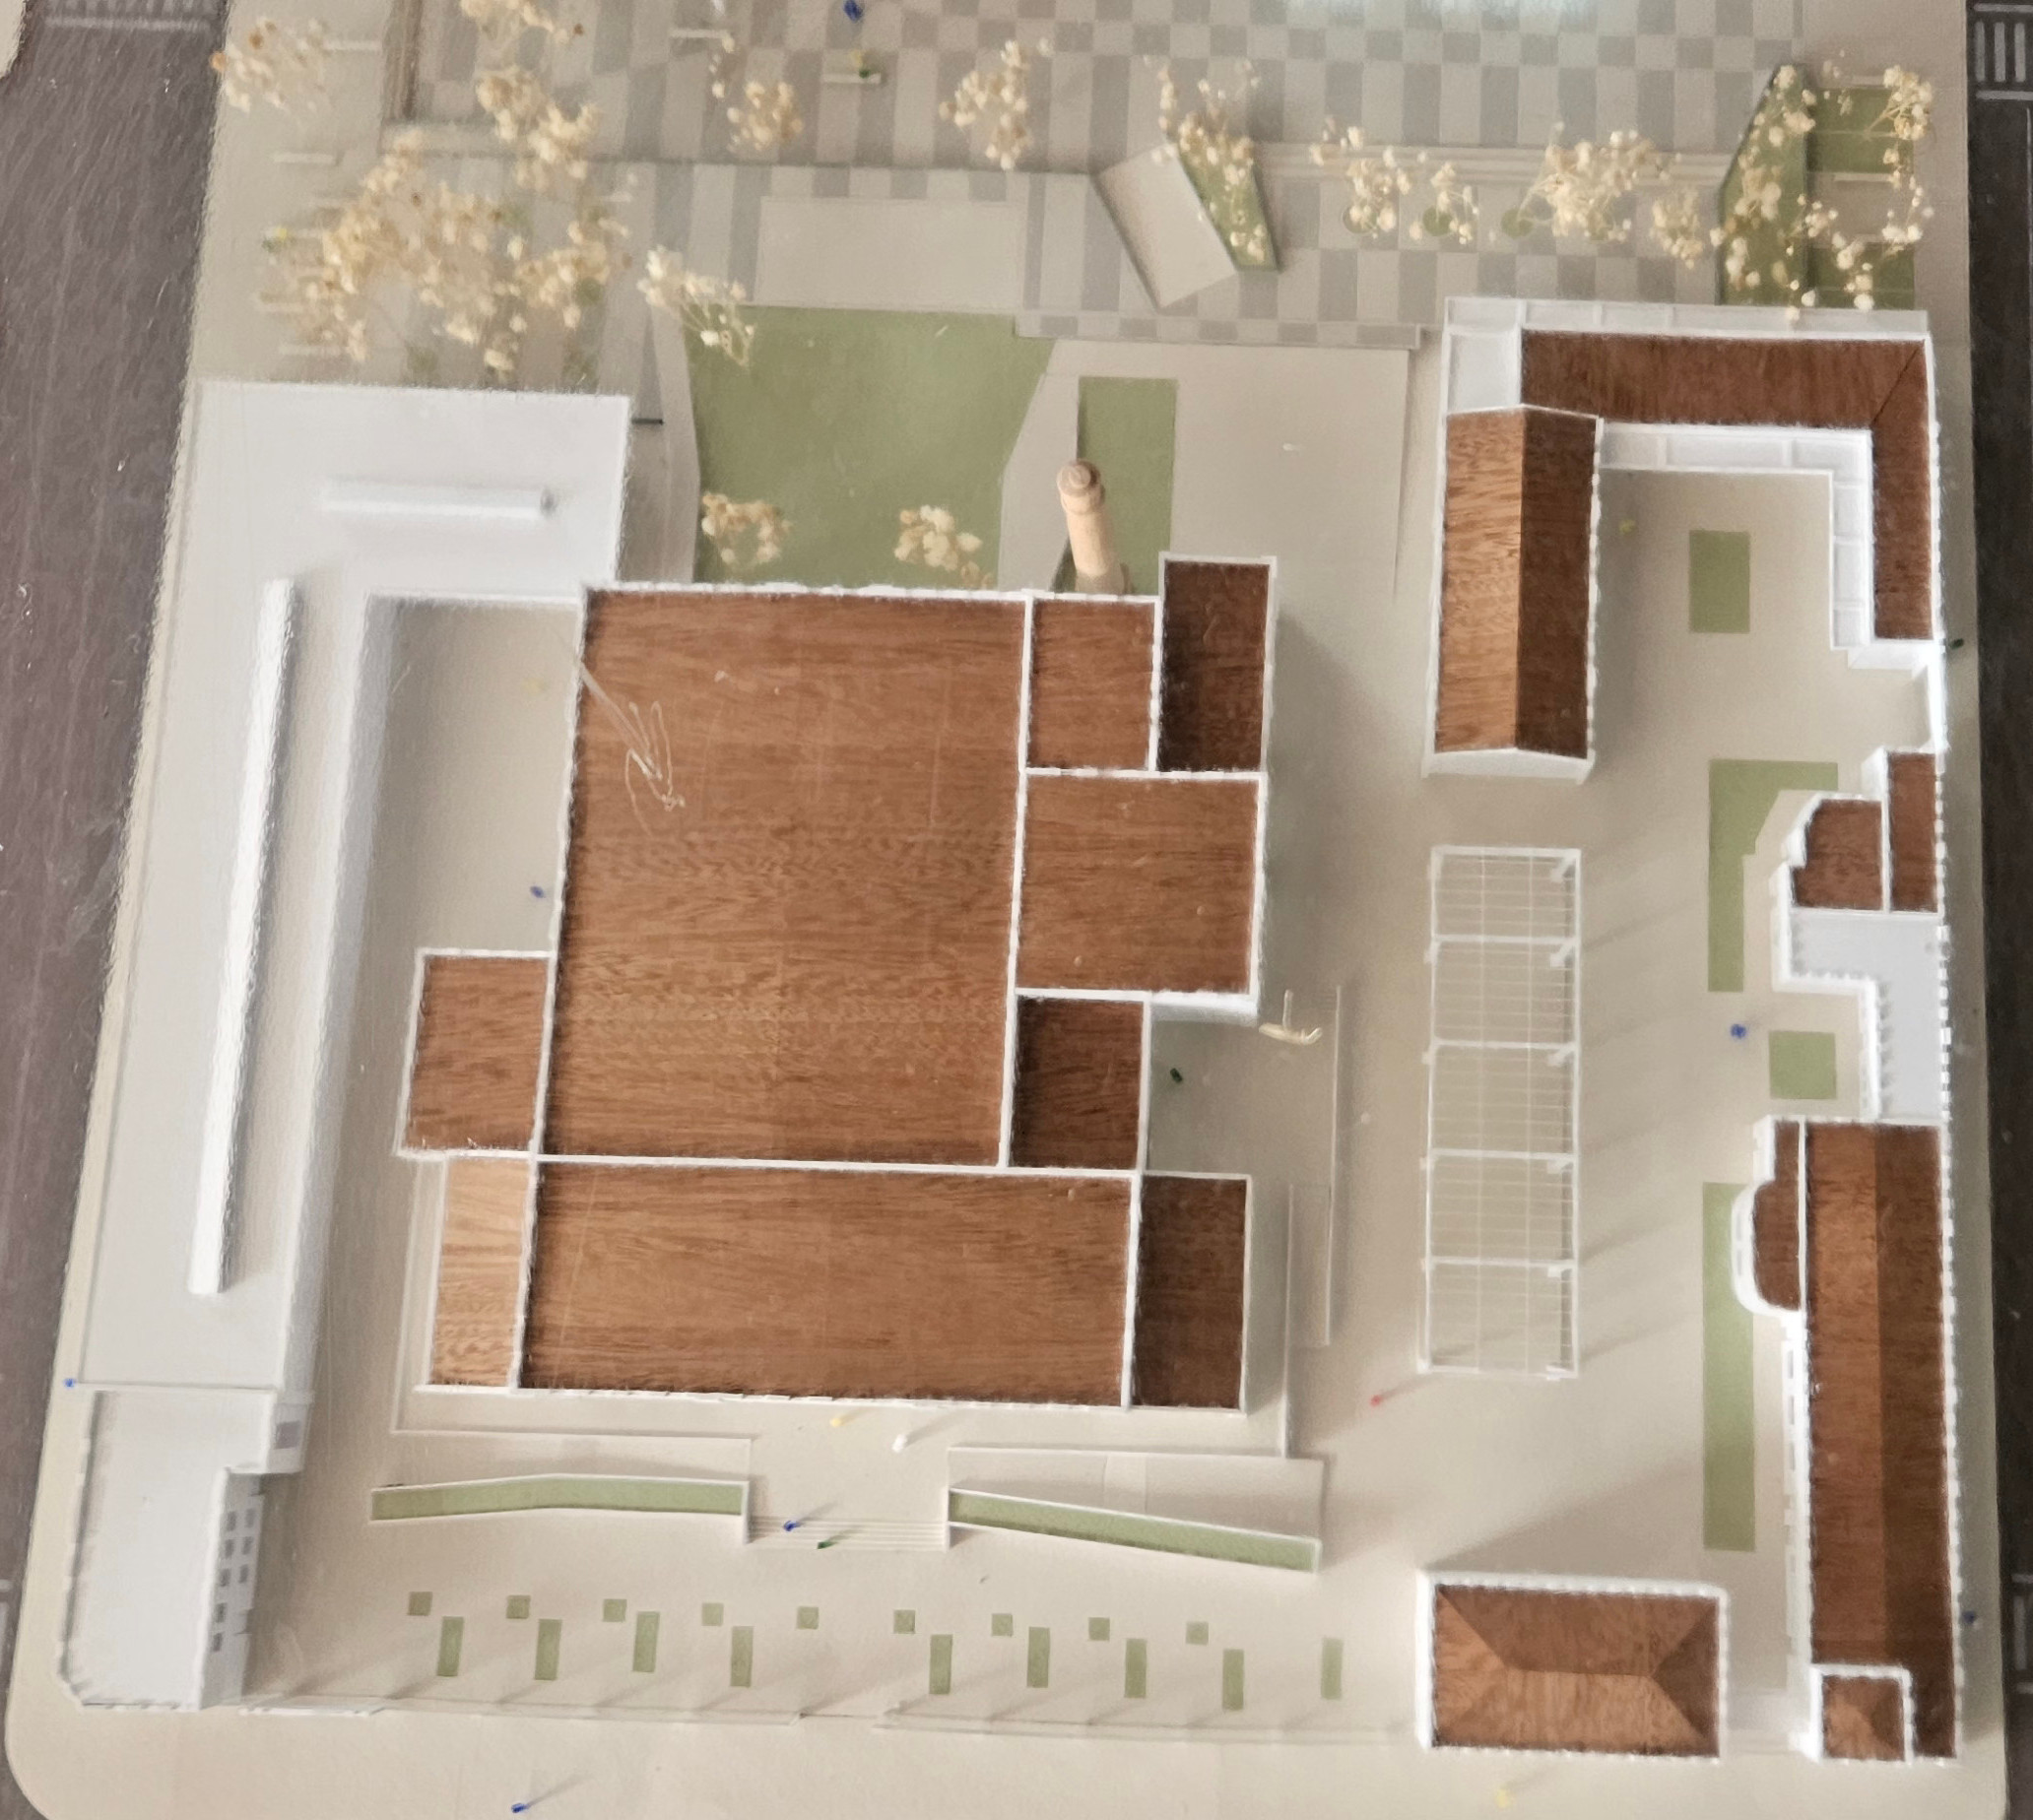
\includegraphics{../../Photos/model-02.jpg}};
	\draw[step=1.0, gray, thin] (0, 0) grid (100, 65);
	\draw[step=10, red, thin] (0, 0) grid (100, 65);

	\draw[fill=yell, thin, nearly opaque] (46.5, 44.3) -- (62.5, 44) -- (61.5, 23.2)
		-- (45, 24) -- cycle;
	\node[font=\fontsize{60}{12}\selectfont] at (54, 34) {Biblioteca};

	\draw[fill=oran, thin, nearly opaque] (62.4, 37.7) -- (71, 37.5) -- (70.5, 29.5)
		-- (62, 30) -- cycle;
	\node[font=\fontsize{60}{12}\selectfont, align=center] at (66.5, 34)
		{Aud. \\ Central};

\end{tikzpicture}
\end{document}
